\RequirePackage[hyphens]{url}
\documentclass[12pt]{IEEEtran}
\usepackage{graphicx}
\usepackage{amsmath}
\usepackage{pgfplots}
\usepackage{cite}
\usepackage{caption}
\usepackage{algorithm}
\usepackage{algpseudocode}
\usepackage{amsfonts}
\markboth{CPSC 530 - Information Theory and Security - Final Report - Group 17}{Last Name \MakeLowercase{\textit{et al.}}: Title}
\usepackage{filecontents}
% Insert references here
\begin{filecontents*}{references.bib}
@masterthesis{Sjostrand,
	title	= {A study in compression algorithms},
	school	= {Blekinge Institue of Technology},
	author	= {Sjostrand, Mattias Hakansson},
	year	= {2005},
	url	= {http://bth.diva-portal.org/smash/record.jsf?pid=diva2:830266}
}
@misc{GitHub,
	title	= {CPSC 530 Project Repository},
	url	= {https://github.com/Aidenwjt/CPSC-530-PROJECT}
}
@misc{Huffman,
	title	= {Huffman Coding Implementation},
	url	= {https://github.com/e-hengirmen/Huffman-Coding}
}
@misc{code1,
	title	= {Key Value Dictionary Implementation},
	url	= {https://gist.githubusercontent.com/kylef/86784/raw/fe97567ec9baf5c0dce3c7fcbec948e21dfcce09/dict.c}
}
@misc{code2,
	title	= {Binary Tree Implementation},
	url	= {https://www.programiz.com/dsa/binary-tree}
}
@misc{code3,
	title	= {Copy Integer Array Implementation},
	url	= {https://stackoverflow.com/questions/8287109/how-to-copy-one-integer-array-to-another}
}
\end{filecontents*}

\newcommand{\Aiden}{Aiden Taylor - B.Sc. in Computer Science}
\newcommand{\Noah}{Noah Pinel - B.Sc. in Computer Science}
\newcommand{\Ty}{Ty Irving - B.Sc. in Computer Science}

\definecolor{mybabyblue}{RGB}{140,216,231}
\definecolor{mysoftgreen}{RGB}{120,233,212}

\begin{document}
\title{The Implementation and Comparison of the BCCBT Data Compression Algorithm}
%\author{
%\begin{tabular}{l}
%    \Aiden \\ \Noah\\ \Ty\\ 
%\end{tabular}}
\author{
    \Aiden \\ \Noah\\ \Ty\\ 
}
\date{Apr. 12th, 2023}

\maketitle

\begin{abstract}
%Elaborate upon each major aspect of the paper.
When storing, transferring, or receiving files it is important to have data compression algorithms to make
these processes easier and more efficient. In our project we dive into the actual implementation
of a proposed data compression algorithm, and use certain factors of comparison to guage our implementation
against other open source data compression algorithms.
\end{abstract}

\section{Introduction}
%Provides the context and motivates the topic. It introduces the paper/research that is the basis of the project.
The purpose of this paper is to take a deeper dive into the implementation and comparison of data compression
algorithms. In the modern age, data compression algorithms have become an integral part of our daily lives.
These algorithms help us save space on our hard drives, use up less bandwidth,
speed up communications, and so much more. \\

Unfortunately, all these great benefits do
not come without costs. In reality, data compression algorithms can be incredibly difficult to devise, and even
more difficult to implement. 
Devising a data compression algorithm requires rigorous mathematical justifications for all the processes taken, and
then implementing a data compression algorithm requires intimate knowledge of optimization and memory management
techniques. \\

Once a data compression algorithm is devised and implemented, it is important to see how it
stacks up against the other readily available options. No one algorithm excels at compressing every
type of data \cite{Sjostrand}, so comparing a data compression algorithm against other available options
can highlight the areas where an algorithm exceeds, or highlight the areas where it falls behind. The most important factors 
of comparisons to note are the compression and decompression times, and how much of the original file
the algorithm is able to save without losing any data from the source file.\\

In this study, we decided to focus on the already devised Bit Code Complete Binary Tree (BCCBT) data compression algorithm
which was
proposed by Mattias Håkansson Sjöstrand in his 2005 Master's Thesis \cite{Sjostrand}.
Using the pseudocode provided in
Sjöstrand's thesis, we first implemented the algorithm, which was written mainly in C with some accompanying Python scripts, then we used four factors of comparison
to guage our implementation against two other open source data compression algorithms. Finally, from these comparisons, we made conclusions about the effectiveness of our implementation.

\section{Proposed Work}
%Describes the proposed work and evaluation framework (e.g. experiments, data analysis, statistical tests, mathematical proof..).
Our proposed work is intended to be a re-implementation of the BCCBT algorithm proposed by Sjöstrand for data compression. 
To achieve this goal, we have proposed a three-part effort that involves implementing the BCCBT algorithm, testing its performance on 
various sized text files, and evaluating its effectiveness compared to state-of-the-art compression algorithms. By undertaking this 
project, we aim to contribute to the field of data compression and provide insights into the effectiveness of the BCCBT algorithm. \\

To begin our work, we first configured the necessary software to emulate the BCCBT algorithm. This involved developing a collection of Python 
programs and a main C program to enable us to accurately simulate the algorithm's behavior.
Next, we evaluated the performance of the BCCBT algorithm by conducting tests to measure its 
compression effectiveness against two other popular compression algorithms, Huffman and Gzip. 
To perform these tests, we used a diverse set of six .txt files of varying sizes, ranging from 1MB to 80MB. 
By comparing the compression ratios and processing speeds of each algorithm, we were able to determine the effectiveness of the BCCBT algorithm. \\

Finally, we assessed the effectiveness of our implementation by replicating the evaluation process described in the original paper \cite{Sjostrand}. 
Using the same metrics as the original work, we measured various compression thresholds to compare our results with his. 
Overall, this framework allowed for us to accurately develop and test our results seamlessly while still being precise with our scientific approach.
\section{Evaluation}
%Implementation and Experiments: what you actually did (objectives, choices, data, and final analysis of results).
%Base comparison: (what is a comparable work, and relating your work to existing works).
%Developed software and how it can be evaluated.

\subsection{Implementation}
Our implementation of the BCCBT data compression algorithm closely follows the pseudocode provided in Sjöstrand's thesis,
which can observed in Figure 1.
\begin{figure}[h]
\centering
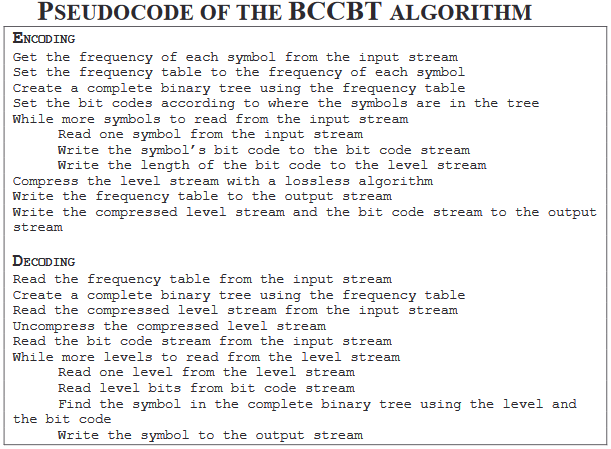
\includegraphics[scale=0.55]{../presentation/images/pseudocode.PNG}
\caption{Pseudocode from \cite{Sjostrand}}
\end{figure}
From a high level perspective, our implementation of the BCCBT data compression algorithm can essentially be split up into two different sections,
being the implementation of the Complete Binary Tree section, and the implementation of the Encoding and Decoding of files section.
To help guide the understanding of both these sections we have decided to use example 3-11 from the thesis as this example does an excellent job of explaining
how the BCCBT algorithm works at a high level \cite{Sjostrand}, and can give the reader a clearer understanding of how we actually implemented the algorithm
without the needing to see any code.
Finally, at the end of this section, we will briefly discuss the developed software and give reference on how it can be evaluated. \\

\subsubsection{Complete Binary Tree} 
To start example 3-11, suppose that we have an alphabet 
\[\Sigma = \{a,b,c,d,e,f,g,h\}\]
taken from a source file where each symbol has a frequency
given from the table in Figure 2.
\begin{figure}
\centering
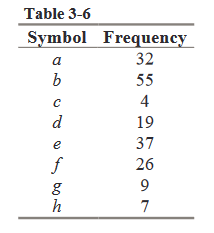
\includegraphics[scale=0.60]{../presentation/images/frequencytable.PNG}
\caption{Frequency table from example 3-11 \cite{Sjostrand}}
\end{figure}
Looking at the pseudocode, we now want to construct a complete binary tree that will allow us to set the bit codes of each
symbol based on its location in the binary tree. \\

Before we construct the complete binary tree in this example, lets first note some of
important properties of a complete binary tree:
\begin{itemize}
\item All levels of the binary tree are completely full except possibly the lowest level.
\item The binary tree is filled in from top down and left to right at each level.
\item The number of nodes in the binary tree at level $n$ is $2^n$ ($n \in \mathbb{Z}_9$).
\end{itemize}
The last of these properties is really only important for Theorem 3-1 in the thesis \cite{Sjostrand}, however we do not actually use
this Theorem's optimization technique in our implementation so we will ignore it for now. \\

Now back to the example, the psuedocode says to construct the complete
binary tree using the frequency table. This means that we insert the highest frequency symbol $b$ as the root node, then at the
next level of the binary tree starting from the left we fill in the next highest frequency symbol $e$, then moving one node to
the right at the same level we fill in the next highest frequency symbol $a$, and so on. Continuing this process until there are no
more unique symbols to add into the binary tree will result in the binary tree having the required properties of a complete binary tree,
as desired
The complete binary tree generated in this example can be seen in Figure 3.\\
\begin{figure}
\centering
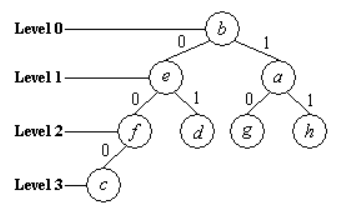
\includegraphics[scale=0.6]{../presentation/images/completebinarytree.PNG}
\caption{Complete binary tree from example 3-11 \cite{Sjostrand}}
\end{figure}

\subsubsection{Encoding and Decoding}
Below we will demonstrate the three main steps in encoding and decoding using the BCCBT algorithm, it is important
to note that this is merely a toy example for the purpose of understating. \\

Firstly, fix the frequency table from Figure 2, where our new frequency table is ordered from the highest occurrences to lowest.
This will give a better reference when we begin encoding and decoding strings of text.
\begin{figure}[h]
    \centering
    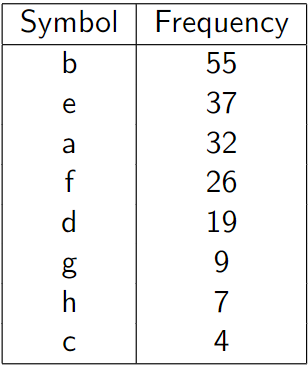
\includegraphics[scale=0.35]{../presentation/images/freqtbl.png}
    \captionsetup{justification=centering}
    \caption{Frequency table for symbols}
\end{figure}
\\
Note that if we were to traverse the binary tree that we constructed 
and record the symbols that we encounter as we move from left to right, we would obtain the same sequence of symbols as in the original 
frequency table, provided that the tree has been constructed correctly. Below is the corresponding complete binary tree that we will use 
for this demonstration.
\begin{figure}[h]
    \centering
    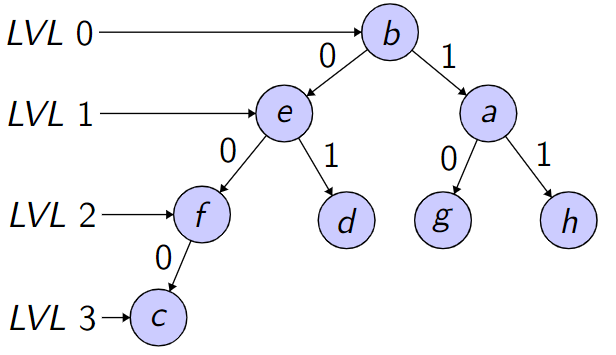
\includegraphics[scale=0.35]{../presentation/images/bintree.png}
    \captionsetup{justification=centering}
    \caption{Complete binary tree}
\end{figure}
\\
We have now set the bedrock for everything we need to do with our algorithm, whether it be encoding a string, or decoding 
an encoded string. Before we begin encoding, we first need to establish the last piece of the puzzle, that is, the corresponding 
bit codes for the symbols in $\Sigma$. In order to generate the bitcodes for each node in the tree, we must follow some simple steps
to retrieve them. The steps are
\begin{enumerate}
	\item Position yourself at the root node of the tree
	\item Traverse the tree, keeping note of the weights on every edge that was needed to get to your desired symbol
	\item After reaching your symbol, you should have a string of 1's and 0's that act like coordinates for finding the specific node.
\end{enumerate}
So, for example, if we wanted to find the bitcode for the symbol $h$, we start at the root of our tree and traverse
two right edges, $b$ to $a$ and then $a$ to $h$, concatenating the edge weights we saw in our walk we get the bitcode 11 for node $h$. Lastly, before we move on
it is important to note that the root of the binary tree i.e. the most occurring symbol in $\Sigma$, takes no bitcode value and instead is set to null.
Below is the complete table of bitcodes corresponding to all of our symbols in $\Sigma$.\\
\begin{center}
	\begin{tabular}{|c|c|c|c|c|c|c|c|}
		\hline
		\multicolumn{8}{|c|}{BIT CODES} \\
		\hline
		a & b & c & d & e & f & g & h \\
		\hline
		1  & NULL  & 000  & 01  & 0  & 00  & 10  & 11\\
		\hline
	\end{tabular}\\
	\vspace{0.1in}
	Table of bitcodes
\end{center}
This is good and all, but unfortunately, 
there is a problem with the current bit codes that we have constructed from the complete binary tree. They are not sufficient to encode a string because they are not 
uniquely decodable. This means that a stranger looking at the complete binary tree alone would not be able to determine what the following string 111 corresponds to - 
is it three $a$'s or one $h$ followed by an $a$? This lack of uniqueness means that we cannot decode the encoded string without losing information, and if we cannot decode it,
we cannot expect a computer to be able to do so either. Therefore, we need to modify our bit codes to ensure that they are uniquely decodable. \\

The way the BCCBT algorithm 
handles this is quite clever, as it provids a simple yet elegant tactic that will allow us to uniquely decode. What we do is simply take the corresponding level where the symbol node 
lays in the tree, and prepend that level value to the bitcode, so for example, $h$ had a bitcode 11, but after making this change the bitcode is now [2]11, So with this, there
can't be any confusion, as you will have to note that the symbol is on the second level of our tree, and then take the walk given, 1, then 1 again, and then arrive at $h$! This is everything we need,
and we can now generate uniquely decodable strings that will allow for lossless decoding.\\

Lets encode the word `edge'. Using our binary tree we take note of the following 3 bitcodes that are generated by iterating the 
simple bitcode generation steps.
\begin{enumerate}
	\item $e$ $\rightarrow$ [1]0
	\item $d$ $\rightarrow$ [2]01
	\item $g$ $\rightarrow$ [2]10
\end{enumerate}
we now have our encoded string
\begin{equation*}
	\text{`edge' } \rightarrow [1]0[2]01[2]10[1]0
\end{equation*}
we can now proceed to simulate the decoding of this string.\\

To decode the encoded string [1]0[2]01[2]10[1]0, we first create a complete binary tree, which we'll need for decoding. 
The decoding process is almost as simple as encoding. We begin by examining the first level token, [1], and extracting all the 
bitcodes between this level token and the next one. In this case, we find the code 0 and stop grouping since the next character is a 
level bracket. This gives us our first encoding block, [1]0. We know with certainty that the desired symbol is in the first level, and we can 
find it by traversing one 0 edge down. In this case, we land on the symbol $e$. We repeat this process for the rest of the string, resulting in the 
following decoding mappings:
\begin{enumerate}
	\item[1)] [1]0 $\rightarrow$ $e$
	\item[2)] [2]01 $\rightarrow$ $d$
	\item[3)] [2]10 $\rightarrow$ $g$
	\item[4)] [1]0 $\rightarrow$ $e$
\end{enumerate}
which tells us that our decoded string is 
\begin{equation*}
	[1]0[2]01[2]10[1]0 \rightarrow \text{`edge' }
\end{equation*}
and with that we conclude this thorough example of how the BCCBT algorithm goes about encoding and decoding strings of text.\\

\subsubsection{Developed Software}
\begin{itemize}
\item \textbf{bccbt.c:} This file contains the implementation for both constructing and searching the Complete Binary Tree,
which in turn contains the implementation for encoding symbols to character arrays of 1's and 0's,
and decoding character arrays of 1's and 0's into their corresponding symbols.
\item \textbf{bitarray.py:} This file contains the implementation for converting a character array of 1's and 0's
to actual bits that can be written to a binary file.
\item \textbf{bitpull.py:} This file contains the implementation for converting a binary file to a character
array of 1's and 0's.
\item \textbf{Makefile:} This file contains tests with the required sequence of commands needed
in order to properly execute our implementation.
\end{itemize}
Our software can simply be evaluated through the Makefile which contains pre-built tests for various different file sizes,
where each of these tests can be edited at the discretion of the user. All of this code can be found in our public
GitHub repository where the link can be found in our references \cite{GitHub}.

\subsection{Experiments}
In order to effectively analyze the BCCBT algorithm we had to 
find two other comparable open source compression algorithms to test against. 
The factors of comparison that we used to actually compare the three algorithms are as follows:
\begin{enumerate}
	\item Compression Time
	\item Decompression Time
   	\item Saving \% = $\frac{Orig\ File\ Size - Compressed\ File\ Size}{Orig\ File\ Size}$
    	\item Compression Ratio = $\frac{Compressed\ File\ Size}{Original\ File\ Size}$
\end{enumerate}
Using these factors of comparison enabled us to test whether or not the BCCBT algorithm was effective 
for compressing files of differing sizes. Note that the following results are given from our implementation
of the BCCBT algorithm and may not accurately depict the results of the original implementation.
\resizebox*{2.8in}{2.5in}{
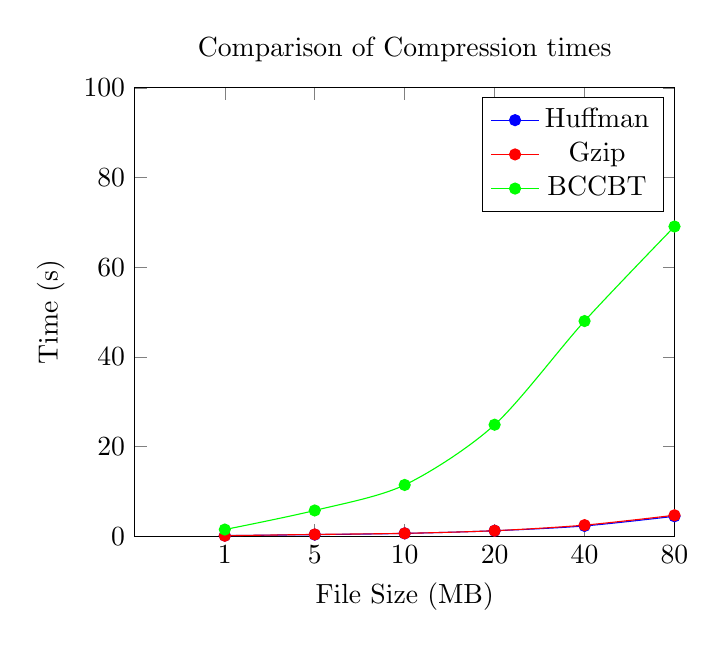
\begin{tikzpicture}
	\begin{axis}[
		xlabel=File Size (MB),
		ylabel=Time (s),
		xmin=0, xmax=6,
		ymin=0, ymax=100,
		xtick={1,2,3,4,5,6},
		xticklabels={1,5,10,20,40,80},   % <---
		ytick={0,20,...,100},
		title={Comparison of Compression times}
				]
	\addplot[smooth,mark=*,blue] plot coordinates {
		(1,0.129)(2,0.351)(3,0.625)(4,1.216)(5,2.293)(6,4.443)
	};
	\addlegendentry{Huffman}
	
	\addplot[smooth,color=red,mark=*]
		plot coordinates {
			(1,0.107)(2,0.394)(3,0.638)(4, 1.228)(5,2.472)(6, 4.671)
	
		};
	\addlegendentry{Gzip}
	\addplot[smooth,color=green,mark=*]
		plot coordinates {
			(1,1.485)(2,5.739)(3,11.430)(4,24.864)(5,47.988)(6, 69.076)
		};
	\addlegendentry{BCCBT}
	
	\end{axis}
\end{tikzpicture}}\\
These first results indicate that although for low file sizes the compression time is quite similar,
as the file size gets bigger the compression time exponentially grows and the gap between
both Huffman and GZip gets bigger and bigger. This result indicates that
it would not be practical, or in your best interest to use our implementatoin on file sizes above 1MB,
as the other two algorithms greatly exceed our implementation is compression time. \\

Not all hope is lost for our implementation though.
Through our tests we were able to find that the compression times of our
implementation of the BCCBT algorithm were slower than GZip and Huffman because of how we
populate and traverse through our complete binary tree. In our implementation we are actually traversing the tree recursively rather than
iteratively which can heavily impact the run time, making our implementation much
slower when compared to the Huffman and Gzip compression times.
\resizebox*{2.8in}{2.5in}{
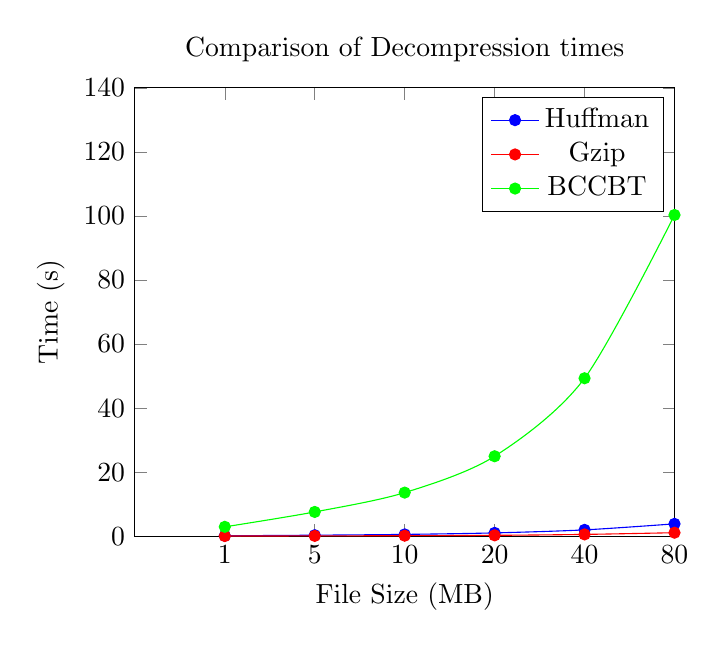
\begin{tikzpicture}
	\begin{axis}[
		xlabel=File Size (MB),
		ylabel=Time (s),
		xmin=0, xmax=6,
		ymin=0, ymax=140,
		xtick={1,2,3,4,5,6},
		xticklabels={1,5,10,20,40,80},   % <---
		ytick={0,20,...,140},
		title={Comparison of Decompression times}
				]
	\addplot[smooth,mark=*,blue] plot coordinates {
		(1,0.123)(2,0.313)(3,0.561)(4,1.030)(5,1.974)(6, 3.853)
	};
	\addlegendentry{Huffman}
	\addplot[smooth,color=red,mark=*]
		plot coordinates {
			(1,0.045)(2,0.092)(3,0.154)(4, 0.269)(5,0.557)(6, 1.091)
	
		};
	\addlegendentry{Gzip}
	\addplot[smooth,color=green,mark=*]
		plot coordinates {
			(1,2.92)(2,7.576)(3,13.611)(4,24.964)(5, 49.321)(6, 100.311)
		};
	\addlegendentry{BCCBT}
	\end{axis}
\end{tikzpicture}}\\
The results for the comparision of the decompression times are quite similar to the 
compression times mainly because decompression in this algorithm uses very similar functions to the 
functions used in compression. This graph again illustrates the problem we faced with the optimization of
the compression and decompression functions in our implementation of the BCCBT algorithm, while at larger
file sizes.\\
\resizebox*{2.8in}{2.5in}{
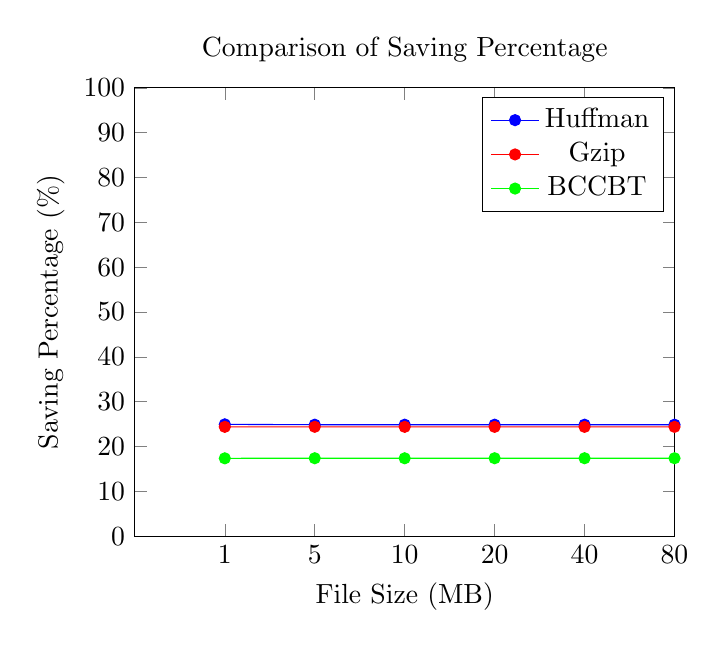
\begin{tikzpicture}
	\begin{axis}[
		xlabel=File Size (MB),
		ylabel=Saving Percentage (\%),
		xmin=0, xmax=6,
		ymin=0, ymax=100,
		xtick={1,2,3,4,5,6},
		xticklabels={1,5,10,20,40,80},   % <---
		ytick={0,10,...,100},
		title={Comparison of Saving Percentage}
				]
	\addplot[smooth,mark=*,blue] plot coordinates {
		(1,24.95)(2,24.87)(3,24.87)(4,24.87)(5,24.87)(6,24.87)
	};
	\addlegendentry{Huffman}
	
	\addplot[smooth,color=red,mark=*]
		plot coordinates {
			(1,24.39)(2,24.40)(3,24.39)(4,24.39)(5,24.39)(6,24.39)
		};
	\addlegendentry{Gzip}
	\addplot[smooth,color=green,mark=*]
		plot coordinates {
			(1,17.37)(2,17.39)(3,17.38)(4,17.39)(5,17.39)(6,17.39)
		};
	\addlegendentry{BCCBT}
	
	\end{axis}
\end{tikzpicture}}\\
The graph above demonstrates the saving percentage in \%, which shows the 
comparision of the different algorithms for compression and the overall
effectiveness of each algorithm depending on file size. This demonstrates that
the saving percentage is linear and that the gap between the algorithms does not
exponentially grow like in the compression and decompression times.

\resizebox*{2.8in}{2.5in}{
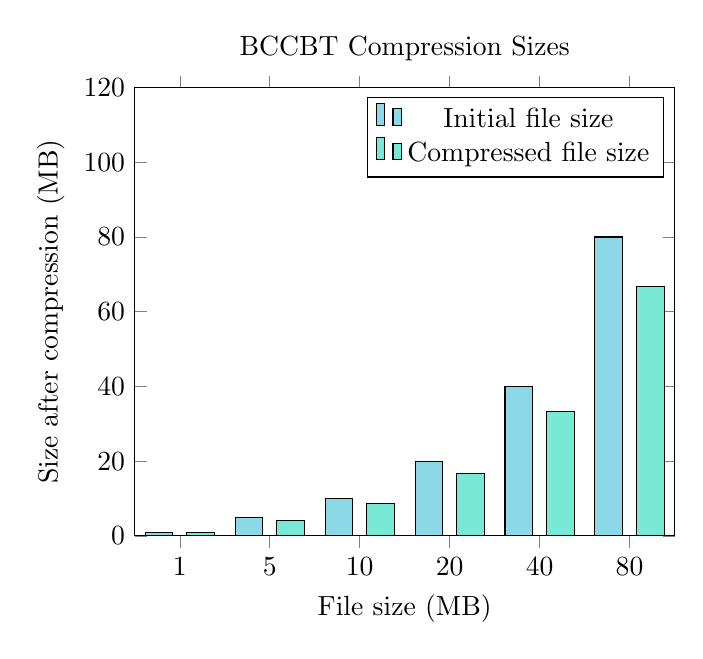
\begin{tikzpicture}
	\begin{axis}[
		title={BCCBT Compression Sizes},
		xlabel={File size (MB)},
		ylabel={Size after compression (MB)},
		ymin=0, ymax=120,
		ytick={0,20,40,60,80,100,120},
		xtick={1,2,3,4,5,6},
		xticklabels={1,5, 10, 20, 40, 80},
		ybar=5pt,
		bar width=10pt,
	]
	
	\addplot[
		fill=mybabyblue,
		]
		coordinates {
		(1,1)(2,5)(3,10)(4,20)(5,40)(6,80)
		};
		\addlegendentry{Initial file size}
		
	\addplot[
		fill=mysoftgreen,
		]
		coordinates {
		(1,0.8)(2,4.17)(3,8.6)(4,16.6)(5,33.3)(6,66.7)
		};
		\addlegendentry{Compressed file size}
	\end{axis}
\end{tikzpicture}}

\resizebox*{2.8in}{2.5in}{
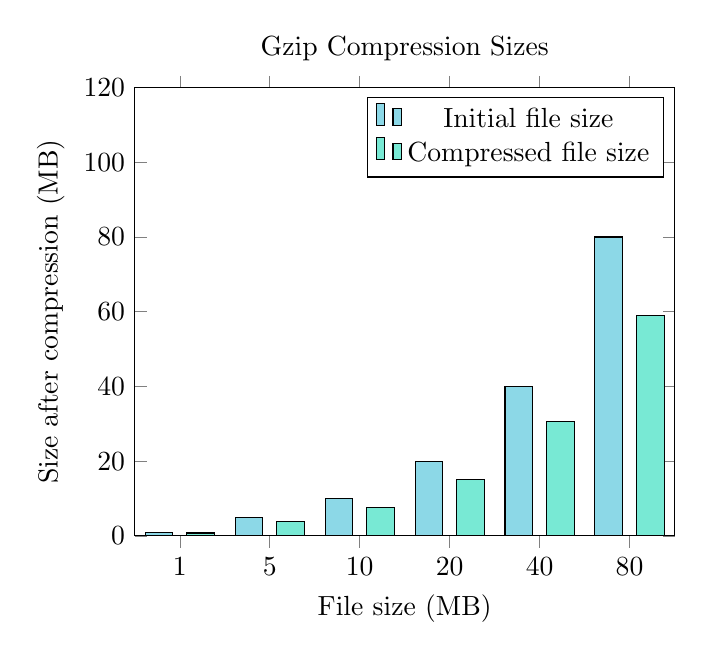
\begin{tikzpicture}
\begin{axis}[
	title={Gzip Compression Sizes},
	xlabel={File size (MB)},
	ylabel={Size after compression (MB)},
	ymin=0, ymax=120,
	ytick={0,20,40,60,80,100,120},
	xtick={1,2,3,4,5,6},
	xticklabels={1,5, 10, 20, 40, 80},
	ybar=5pt,
	bar width=10pt,
]

\addplot[
	fill=mybabyblue,
	]
	coordinates {
	(1,1)(2,5)(3,10)(4,20)(5,40)(6,80)
	};
	\addlegendentry{Initial file size}
	
\addplot[
	fill=mysoftgreen,
	]
	coordinates {
	(1,0.76)(2,3.8)(3,7.6)(4,15.2)(5,30.5)(6,59)
	};
	\addlegendentry{Compressed file size}
\end{axis}
\end{tikzpicture}}

\resizebox*{2.8in}{2.5in}{
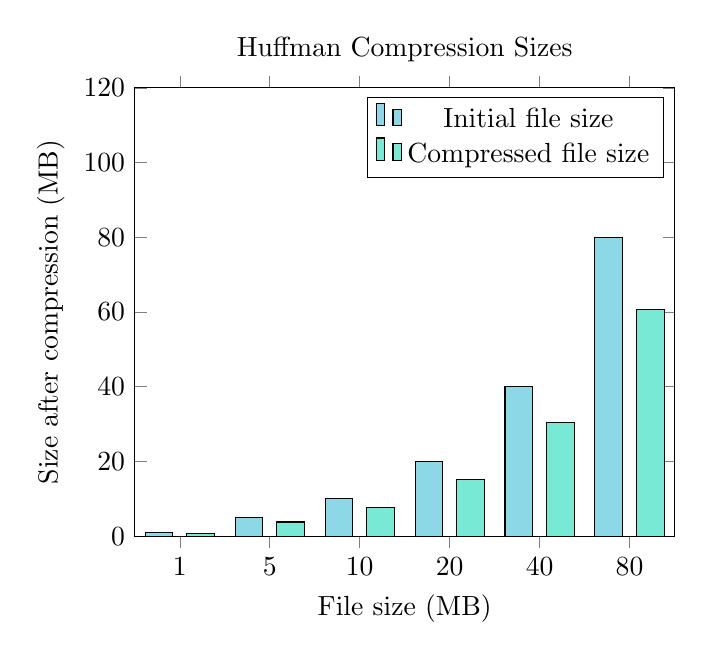
\begin{tikzpicture}
\begin{axis}[
	title={Huffman Compression Sizes},
	xlabel={File size (MB)},
	ylabel={Size after compression (MB)},
	ymin=0, ymax=120,
	ytick={0,20,40,60,80,100,120},
	xtick={1,2,3,4,5,6},
	xticklabels={1,5, 10, 20, 40, 80},
	ybar=5pt,
	bar width=10pt,
]

\addplot[
	fill=mybabyblue,
	]
	coordinates {
	(1,1)(2,5)(3,10)(4,20)(5,40)(6,80)
	};
	\addlegendentry{Initial file size}
	
\addplot[
	fill=mysoftgreen,
	]
	coordinates {
	(1,0.758)(2,3.79)(3,7.58)(4,15.17)(5,30.35)(6,60.7)
	};
	\addlegendentry{Compressed file size}
\end{axis}
\end{tikzpicture}}\\
The compression size graphs for the Huffman, Gzip, and BCCBT all show that no matter
what the file size is, the amount the file size is being reduced stays linear. Another
important part to note about this graph is that the BCCBT algorithm does not make the compressed file size
as small as the other compression algorithms, further indicating how the algorithm is not as 
efficient as the other open source algorithms that we compared our implementation against. \\

In conclusion,
based on the experiment results that have been presented, the BCCBT algorithm is an efficient 
compression algorithm, however, our implementation of the code that compresses and decompresses the bitcodes,
levels, and frequency files make the distinction of usability clear. Our implementation of the 
BCCBT algorithm performs much slower than the two open source algorithms, showing that it is less practical for large file sizes.

\section{Findings and Conclusion}
Overall, the results of our experiments show that the BCCBT algorithm itself should only perform slightly worse
when compared to the open source compression algorithms that were used in comparision.
We must note that the results for the compression and decompression times were heavily influenced by the time constraints of this project
as we had to implement the whole algorithm from scratch, and hence little focus was put into the optimization of our implementation.
The results for the compression sizes tell a more convincing story as they were quite similar to 
the other two algorithms used in comparison. Therefore, we can say with confidence that the BCCBT data compression algorithm
is actually an effective algorithm that can be used in practical scenarios, given that you optimize the compression and decompression times.

\section{Planning and Execution}
%Compares the final work with the project proposal: comments on if the stated goals have been achieved, and if not, outlines the challenges.
%Outlines contributions of group members including, ideas, implementation, research, writing report.\\

When comparing the final result of our project with our project proposal, it is clear to see that we were able to effectively
achieve our main goal of implementing the BCCBT algorithm in order to compare it against other
compression algorithms. \\

The biggest challenge we faced in our
project was simply just the implementation of the BCCBT algorithm since we had to write the compression and 
decompression code from scratch.
This took some time which resulted in code that was not as optimized as it could be. 
Given more time, or given the opportunity for future work, we do believe that we could yield better results by simply implementing more optimized code. \\

The work throughout this project was evenly split up between all group members.
All group members worked on the implementation of the algorithm by splitting it up
into encoding, decoding, and the setting up of the complete binary tree and frequency table functionalities.
The presentation and supporting papers were evenly split up as well, with each group member working on their assigned section
representing what they focused on during the implementation and research.

\phantom{\cite{Huffman}\cite{code1}\cite{code2}\cite{code3}}

\bibliographystyle{IEEEtran}
\bibliography{references}

\end{document}
